\documentclass[twoside]{report}
\usepackage{bm}
\usepackage{ifthen}
\bibliographystyle{plain}
\newcommand{\diff}{\mbox{$\mathrm{d}$}}     % Differential d (for differential operators)
\newcommand{\norm}[1]{\mbox{$||#1||$}}      % Magnitude/Norm
\newcommand{\ve}[1]{\mbox{$\ifthenelse{     % Vector
    \equal{#1}{\alpha}\or\equal{#1}{\beta}\or\equal{#1}{\gamma}\or\equal{#1}{\delta}\or
    \equal{#1}{\epsilon}\or\equal{#1}{\varepsilon}\or\equal{#1}{\zeta}\or\equal{#1}{\eta}\or
    \equal{#1}{\theta}\or\equal{#1}{\vartheta}\or\equal{#1}{\iota}\or\equal{#1}{\kappa}\or
    \equal{#1}{\lambda}\or\equal{#1}{\mu}\or\equal{#1}{\nu}\or\equal{#1}{\xi}\or
    \equal{#1}{\pi}\or\equal{#1}{\varpi}\or\equal{#1}{\rho}\or\equal{#1}{\varrho}\or
    \equal{#1}{\sigma}\or\equal{#1}{\varsigma}\or\equal{#1}{\tau}\or\equal{#1}{\upsilon}\or
    \equal{#1}{\phi}\or\equal{#1}{\varphi}\or\equal{#1}{\chi}\or\equal{#1}{\psi}\or
    \equal{#1}{\omega}\or\equal{#1}{\Gamma}\or\equal{#1}{\Delta}\or\equal{#1}{\Theta}\or
    \equal{#1}{\Lambda}\or\equal{#1}{\Xi}\or\equal{#1}{\Pi}\or\equal{#1}{\Sigma}\or
    \equal{#1}{\Upsilon}\or\equal{#1}{\Phi}\or\equal{#1}{\Psi}\or\equal{#1}{\Omega}}
    {\bm{#1}}{\mathbf{#1}}$}}
\newcommand{\m}[1]{\ve{#1}}                 % Matrix
\newcommand{\dual}[1]{\mbox{$#1^*$}}        % Dual tensor
\newcommand{\q}[1]{\mbox{$#1$}}             % Quaternion
\newcommand{\qi}{\mbox{$\mathrm{i}$}}       % Quaternion i component
\newcommand{\qj}{\mbox{$\mathrm{j}$}}       % Quaternion j component
\newcommand{\qk}{\mbox{$\mathrm{k}$}}       % Quaternion k component
\newcommand{\zerobox}[1]{%
    \setbox0 = \hbox{\parbox[t][\height][b]{20cm}{#1}}%
    \dp0 = 0pt
    \ht0 = 0pt
    \noindent
    \makebox[0pt][l]{\box0}%
    \ignorespaces
}
\newcounter{flickframe}
\usepackage{fancyhdr}
\pagestyle{fancyplain}
\newcommand{\flickbook}{%
    \fancyhf{}
    \fancyfoot[RO]{\stepcounter{flickframe}
        \zerobox{\rule{2cm}{1.5cm}\\Frame \arabic{flickframe}}}
    \fancyfoot[LE]{y}
}
\flickbook
\fancyhead[RO,LE]{\thepage}
\fancyhead[LO,RE]{\slshape\leftmark}
\fancypagestyle{plain}{%
    \flickbook
    \fancyfoot[CO,CE]{\thepage}
}
\renewcommand{\headrulewidth}{0pt}
\begin{document}
\chapter{Preparation}
The preparatory work for this project splits into two parts:
\begin{itemize}
\item Surveying literature, learning the theoretical background and understanding the existing
    algorithms for my task. The outcome of this preparation is discussed in
    sections~\ref{rigidBodyDynamics} to~\ref{articulatedBodies}.
\item Setting up and learning to use the software environment for development. This is described
    in section~\ref{softwarePreparation}.
\end{itemize}

\section{Rigid body dynamics\label{rigidBodyDynamics}}
On the most theoretical level, a rigid body is a collection of $k$ point masses ($k \ge 3$,
can be infinite) subject to the constraint that the distance between any pair of masses must
remain constant. More conveniently, we can regard a rigid body as an object with a
three-dimensional shape, a non-zero volume and some mass distribution, and assume that it does not
change shape.

At a particular point in time, a rigid body is fully determined by four non-scalar quantities: the
\emph{position} of its centre of mass, its \emph{orientation}, and its \emph{linear} and
\emph{angular velocities}. These values usually change over time. Each of these can be easily
represented as a three-component vector, except for orientation, which is discussed in
section~\ref{quaternions}. By convention a right-handed Cartesian coordinate system is used.

To characterize the body's dynamic behaviour, we also need to know its \emph{inertial mass},
a scalar quantity, and its \emph{moment of inertia}, which is a rank-2 tensor (commonly written
as a $3\times3$ matrix). While the mass stays constant, the moment of inertia may
depend on the body's orientation~-- it is, however, constant when expressed with respect to the
body's \emph{principal axes}~\cite{Feynman:63,Goldstein:80}.

Angular velocity appears to be a straightforward way of describing the body's rotation: the
direction of the vector gives the axis of rotation, while its magnitude is the rate of rotation
in radians per second. Unfortunately, in an asymmetric body, the angular velocity may vary over
time even if there are no external influences on the body, due to an effect
known as \emph{free precession} or \emph{Poinsot motion}~\cite{Goldstein:80,Julian:notes}. It is
therefore more convenient to use \emph{angular momentum} instead, which is conserved in the
absence of torques.

\begin{table}
\renewcommand{\baselinestretch}{1.3}\small\normalsize
\centerline{\begin{tabular}{|l|l|l|}\hline
& \emph{Linear} & \emph{Angular} \\\hline
Resistance to change & Mass $m$ & Moment of inertia \m{I} \\\hline
Stationary state & Centre of mass position \ve{r} & \emph{see section \ref{quaternions}} \\\hline
Velocity & Linear velocity $\ve{v} = \dot{\ve{r}}$ & Angular velocity \ve{\omega} \\\hline
Momentum & Linear momentum     & Angular momentum           \\
         & $\ve{p} = m\ve{v}$ & $\ve{L} = \m{I}\ve{\omega}$\\\hline
External influence & Force $\ve{F} = \dot{\ve{p}}$ & Torque $\ve{\tau} = \dot{\ve{L}}$ \\\hline
\end{tabular}}
\caption{Summary of the physical quantities describing a rigid body.\label{rigidBodySummary}}
\end{table}

Forces and torques acting on a body may change the momenta of a body as described in
table~\ref{rigidBodySummary}. A force \ve{F} may be applied to any point $\ve{r}'$ of
a body. We can treat this as if the force had been applied to the centre of mass \ve{r}, and add
an additional torque given by $\ve{\tau} = (\ve{r}' - \ve{r})\times\ve{F}$. If multiple
forces and torques are applied, all forces (applied to the centre of mass) may be added into
a single vector, and similarly all torques may be added.

To solve the differential equations of motion, forces are integrated over time to find linear
momentum, and torques are integrated to find angular momentum. From each of these we calculate
linear and angular velocities, which are in turn integrated to find the position and orientation
over the course of time. It is important that we integrate over torques (and not angular
accelerations), otherwise the simulation will not correctly conserve angular momentum.

\section{Solving ordinary differential equations (ODEs)\label{solvingODEs}}

Undergraduate mathematics courses cover various methods for solving ODEs analytically.
These work well for simple systems and deliver
an exact solution. For example, if a constant force is applied to a body, its displacement is a
quadratic (parabolic) function of time; if the force is negatively proportional to the
displacement, we observe simple harmonic oscillation. Unfortunately, when systems become
only slightly more complicated, the equations become intractable~-- even a simple pendulum
falls in this category. General solutions can then only be approximated numerically.

\begin{figure}
\centerline{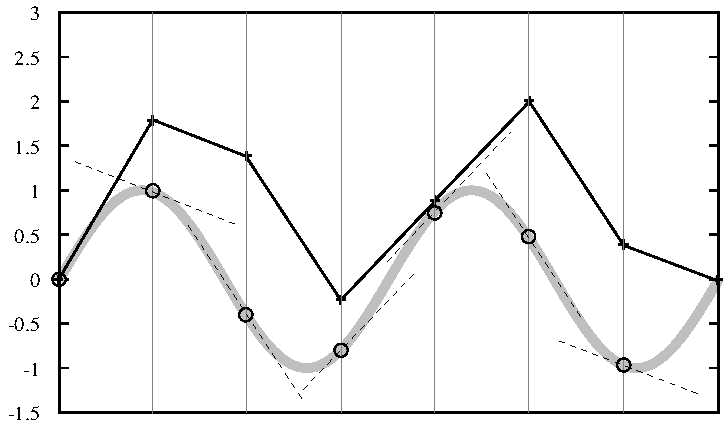
\includegraphics{figures/euler}}
\caption{Demonstration of Euler's method for solving the ODE of simple harmonic oscillation.
    The broad grey line represents the exact solution. At each time step, the method takes the
    derivative (gradient) of the function and uses it to extrapolate linearly.\label{eulersMethod}}
\end{figure}

The general scheme for numerical ODE solvers is to take the value of a function $f(t')$ and its
derivative $\frac{\diff f}{\diff t}(t')$ at some point in time $t'$. From these the algorithm
extrapolates what the value of the function is expected to be some time step $h$ later. The
simplest, most frequently-quoted and worst algorithm for this purpose is Euler's method,
\begin{equation}
f(t'+h) = f(t') + h\frac{\diff f}{\diff t}(t'),
\end{equation}
which performs linear extrapolation. Figure~\ref{eulersMethod} illustrates its operation and the
errors introduced in the solution.

A popular and robust alternative is given by the \emph{Runge-Kutta} family of ODE solvers, which
evaluate $\frac{\diff f}{\diff t}$ at different times and use these values to fit a polynomial
curve to the exact solution over the range of one time step. For example, fourth-order Runge-Kutta
(RK4)~\cite{NRinC} uses four values of the derivative to fit a fourth-order polynomial~-- contrast
this to the first-order polynomial (linear function) used by Euler's method. This amounts to using
the first five terms of the Taylor series of the exact solution, including the $h^4$ term, so
we expect the error in each time step to be $O(h^5)$~-- a minute error even if $h$ is only
moderately small. The step size can be much longer than in Euler's method while achieving the same
accuracy, which makes Runge-Kutta significantly more efficient.

Further improvements can be made by adapting the step size $h$ to the situation. In this project
I chose to use the embedded Cash-Karp/Runge-Kutta method described in~\cite{NRinC}, which uses
six evaluations of the derivative to calculate both a fourth-order and a fifth-order
extrapolation. If the difference between them is small, the total error is likely to be small,
and the next step will be longer. If the absolute difference lies above some threshold, the current
time step is discarded and retried with a smaller $h$. Thus the ODE solver can rapidly skip over
periods in which there is little happening, without sacrificing accuracy in moments of sudden
change.

\section{Quaternions\label{quaternions}}
\subsection{The need for Quaternions}
Besides its position, every rigid body in 3D space may have an orientation. This introduces three
additional degrees of freedom for each stationary body (six if angular velocity is included).
While the position of a body can be neatly represented using Cartesian coordinates, there is
unfortunately no obvious best way of describing an orientation. The most common schemes describe
it in terms of a rotation operation which transforms a vector in the body's local
coordinates into world coordinates (or vice-versa). But again, there are various different
approaches to representing this rotation, all of which have advantages and disadvantages.

\emph{Euler angles} are probably the most intuitive representation of a 3D rotation, describing
it as a series of three rotations about different axes. These axes are fixed by convention, so it
suffices to specify the three angles of rotation. However, this scheme has a number of drawbacks
which are extensively discussed in the literature~\cite{Saunders:PhD,Shoemake:85}: amongst other
things, it is possible that rotation about one of the axes freezes during an animation
(``Gimbal lock'') unless all special cases are handled very carefully.

\emph{Rotation matrices} are commonly used because they are well understood, easily generalize
to other dimensions and allow efficient combination with other linear transformations (scaling
and shearing~-- translation may also be included if homogeneous coordinates are employed).
Unfortunately, many operations required for animation of rotations are awkward to implement
since this representation uses nine numbers (a $3\times3$ matrix) to represent three degrees
of freedom, thus introducing six additional side-conditions which must be maintained.

\emph{Quaternions}~\cite{Shoemake:85,Eberly:01,MathWorld:Quaternion} are a popular alternative
to the two previous schemes, and they are also used extensively in this project.

\subsection{Definition and properties}
Mathematically, quaternions can be regarded as numbers with one real part and three
distinct imaginary parts:
\begin{equation}
\q{q} = q_w + q_x\qi + q_y\qj + q_z\qk
\end{equation}
where $q_w$, $q_x$, $q_y$ and $q_z$ are real-valued numbers and \qi{}, \qj{} and \qk{} satisfy
\begin{equation}
\qi^2 = \qj^2 = \qk^2 = \qi\qj\qk = -1.
\end{equation}
From this follows that
$\qi\qj = -\qj\qi = \qk$ and
$\qj\qk = -\qk\qj = \qi$ and
$\qk\qi = -\qi\qk = \qj$.
Note that multiplication is not commutative.

We will also need the conjugate and the inverse of a quaternion. In analogy to
complex numbers, these are given respectively by
\begin{eqnarray}
\overline{\q{q}} & = & q_w - q_x\qi - q_y\qj - q_z\qk\\
\q{q}^{-1} & = & \frac{\overline{\q{q}}}{\norm{\q{q}}^2}\\
\mathrm{where}\quad&& \norm{q_w + q_x\qi + q_y\qj + q_z\qk} =
    \sqrt{q_w^2 + q_x^2 + q_y^2 + q_z^2}
\end{eqnarray}

Sometimes we will need to relate a 3D vector to a quaternion with zero real part.
For a given vector $\ve{u} = (u_1, u_2, u_3)^T$ we define the corresponding
quaternion to be
\begin{equation}
\label{vectorToQuat}
\tilde{\ve{u}} = u_1\qi + u_2\qj + u_3\qk.
\end{equation}

The complex constants \qi{}, \qj{} and \qk{} are required for the algebra
only, therefore we can represent a quaternion as four numbers $(w,x,y,z)$. It turns out that a
quaternion neatly represents an arbitrary rotation in 3D space (similarly to the way that an
ordinary complex number represents a rotation in the 2D Argand diagram) if we require it to have
unit magnitude ($\norm{\q{q}} = 1$).  This condition reduces the number of degrees of freedom to
three, as required.

Every unit quaternion represents a rotation of angle $\theta$ about an arbitrary axis.
If the axis passes through the origin and has a direction given by the vector
$\ve{a} = (a_1, a_2, a_3)^T$ with $\norm{\ve{a}} = 1$, the quaternion describing
this rotation is
\begin{equation}
\label{quatRotation}
\q{q} = \cos\left(\frac{\theta}{2}\right) + (a_1\qi + a_2\qj +
    a_3\qk) \sin\left(\frac{\theta}{2}\right).
\end{equation}
It can easily be verified that this quaternion always has unit magnitude.
We shall assume throughout this project that the rotation thus described is clockwise (as seen
when looking in the direction of the vector $\ve{a}$) in a right-hand coordinate system,
i.e.\ that it is given by the ``right-hand rule''.

Two rotations can be concatenated by multiplying their quaternions together. Because the order
in which these rotations are applied is significant, this multiplication is not commutative~--
it is, however, associative. By convention the rotations in a product of quaternions are applied
from right to left (see below). The quaternion product is obtained simply by multiplying out the
components, observing the rules for multiplying \qi{}, \qj{} and \qk{}:
\begin{eqnarray}
&& (p_w + p_x\qi + p_y\qj + p_z\qk)(q_w + q_x\qi + q_y\qj + q_z\qk) = \nonumber\\*
&& \quad\quad\quad (p_w q_w - p_x q_x - p_y q_y - p_z q_z) + \nonumber\\*
&& \quad\quad\quad (p_w q_x + p_x q_w + p_y q_z - p_z q_y) \,\qi + \nonumber\\*
&& \quad\quad\quad (p_w q_y + p_y q_w + p_z q_x - p_x q_z) \,\qj + \nonumber\\*
&& \quad\quad\quad (p_w q_z + p_z q_w + p_x q_y - p_y q_x) \,\qk \label{quatProduct}
\end{eqnarray}

We may occasionally find it convenient to write a quaternion as a pair consisting of a scalar
(the real part) and a vector (the three imaginary parts):
$\q{q} = [q_w, \ve{q}_v] = [q_w, (q_x, q_y, q_z)^T]$. Using this notation, we can write the
quaternion product in terms of vector dot and cross products:
\begin{equation} \label{quatProduct2}
\q{p}\q{q} = [p_w,\; \ve{p}_v]\;[q_w,\; \ve{q}_v] =
    [p_w q_w - \ve{p}_v \cdot \ve{q}_v,\;
    p_w \ve{q}_v + q_w \ve{p}_v + \ve{p}_v \times \ve{q}_v]
\end{equation}

To rotate a vector $\ve{v} = (v_1, v_2, v_3)^T$ by a quaternion \q{q}, we first
convert it into its corresponding quaternion $\tilde{\ve{v}}$ as defined in
equation~\ref{vectorToQuat} and then calculate the quaternion product
\begin{equation}
\label{quatTransform}
\tilde{\ve{v}}' = \q{q}\tilde{\ve{v}}\q{q}^{-1}
\end{equation}

If we expand this formula, we find that the real part of the result is always zero, and
that the rotated vector $\ve{v}' = (v_1', v_2', v_3')^T$ corresponds
to $\tilde{\ve{v}}'$ (i.e.\ $\ve{v}'$ is contained in the three complex parts of
the quaternion product).

Some authors, notably Shoemake~\cite{Shoemake:85}, choose to define the product in
equation~\ref{quatTransform} in
the reverse order. The choice is a matter of convention, since it merely changes the effect
of this operation from being a clockwise to a counter-clockwise rotation. We chose the clockwise
convention because it is consistent with the usual definition of the angular velocity vector
in physics.

Observe that under this convention, if \q{q} is itself a product of quaternions, the
result of this transformation is the same as if the rotations denoted to the factors
of \q{q} had been applied starting with the rightmost factor, and continuing from
right to left. To verify that this is the case, the identity
$\overline{\q{p}\, \q{q}} = \q{\overline{q}}\; \q{\overline{p}}$
is useful~\cite{MathWorld:Quaternion}.

\subsection{Quaternion integration}

In a dynamics simulation, the angular momentum of a body is determined by solving the
differential equation of motion, given the torques acting on the body. Similarly, the
orientation of the body should be found by numerical integration, given the angular
velocity. Angular velocity can be represented easily using a 3D vector whose
direction is the axis of rotation and whose magnitude is the scalar quantity (usually in
radians per second). As we have seen, such a concise representation is not possible for
orientation, which leads to some complications.

At this point it might be helpful to consider a geometric view on quaternions. Let us treat
the four components of a quaternion as Cartesian coordinates of a four-dimensional vector
space. The set of unit quaternions is then the surface of a unit hypersphere (also called a
``glome''\cite{MathWorld:4D}) in this vector space. Each point on this hypersphere
corresponds to a particular rotation. It also turns out that each pair of
opposite points on this sphere represent exactly the same rotation; hence all possible
rotations are contained in one hemisphere, no matter where the sphere is cut in half.

The instantaneous rate of change of a quaternion \q{q} over time is usually given
in the literature as
\begin{equation}
\label{quatRateOfChange}
\dot{\q{q}}(t) = \frac{1}{2}\tilde{\ve{\omega}}(t)\q{q}(t)
\end{equation}
where $\tilde{\ve{\omega}}$ is the quaternion corresponding to the angular velocity
vector $\ve{\omega}$. Appendix~\ref{quatIntegrationMagnitude} proves that $\dot{\q{q}}$ is
always orthogonal to $\q{q}$. Geometrically, the space of all possible values of $\dot{\q{q}}$ is
a hyperplane (a three-dimensional subspace) tangential to the sphere at the point $\q{q}$ in
4D space. Thus if $\q{q}$ is a point on the unit sphere, it will still have unit magnitude after
adding an infinitesimal amount $\diff\dot{\q{q}}$; this is exactly what we should expect of the
derivative.

Unfortunately this formula fails in practice since simulations use finite time steps. This
shall be demonstrated using Euler's method; it should, however, be pointed out that more
sophisticated methods like RK4 are equally affected. Consider the value of \q{q} at
the next time step, $\q{q}(t + \Delta t) = \q{q}(t) + \Delta t \dot{\q{q}}(t)$.
For any non-zero $\Delta t$ and $\dot{\q{q}}$ this point will always lie outside the
unit sphere due to the orthogonality of \q{q} and $\dot{\q{q}}$.
This is usually compensated by re-normalizing the quaternion after the ODE solving step.
Geometrically, this re-normalization can be understood as drawing a straight line through
the origin and the point $\q{q}(t) + \Delta t \dot{\q{q}}(t)$,
intersecting this line with the unit sphere and replacing $\q{q}(t + \Delta t)$ by this
point of intersection.

Following the tangent to the sphere is a reasonable approximation to following its curve if the
magnitude of $\Delta t \dot{\q{q}}(t)$ is small compared to the curvature of the sphere.
For large time steps or large magnitudes of \ve{\omega}, however, this gets increasingly
erroneous. Consider the limiting case, a body rotating infinitely fast
($\norm{\ve{\omega}} \rightarrow \infty$): after re-normalisation, $\q{q}$ will have moved merely
a quarter of the way around the unit sphere, while it would have been correct to perform an
infinite number of revolutions around the quaternion sphere.

We can solve this problem by scaling $\Delta\q{q}(t) = \Delta t \dot{\q{q}}(t)$
depending on its magnitude, so that it maps to the correct point on the sphere after
re-normalisation. We can combine this scaling and re-normalisation into one convenient
function to perform a \emph{Qu}at\emph{er}nion inte\emph{g}ration \emph{s}tep, or `Quergs'
in short\footnote{This naming follows the spirit of Shoemake~\cite{Shoemake:85}, whose
``Slerp'' function is an `acronym' of \emph{S}pherical \emph{l}inear int\emph{erp}olation.}:
\begin{equation}
\label{quergs}
\mathrm{Quergs}(\q{q}, \Delta\q{q}) =
    \frac{\q{q} + \tan\left(\norm{\Delta\q{q}}\right)
        \frac{\Delta\q{q}}{\norm{\Delta\q{q}}}}{
    \sqrt{\norm{\q{q}}^2 + \tan^2\left(\norm{\Delta\q{q}}\right)}}
\end{equation}

This formula is derived in appendix~\ref{quatIntegrationDerivation}.
When implementing this formula, care must be taken around the
discontinuities of the $\tan$ function, where numerical instability may occur. These
discontinuities are reached whenever a body performs an odd multiple of half
revolutions during a single time step.

Quergs implements one step of Euler's method for solving an ODE over a quaternion.
Where for Euler's method over an Euclidean vector we would write
$\ve{a}(t + \Delta t) = \ve{a}(t) + \Delta t\,\dot{\ve{a}}(t,\;\ve{a}(t))$,
for quaternions we simply use
$\q{q}(t + \Delta t) = \mathrm{Quergs}(\q{q}(t),\; \Delta t\,\dot{\q{q}}(t)) =
    \mathrm{Quergs}(\q{q}(t),\; \frac{\Delta t}{2}\,\tilde{\ve{\omega}}(t)\q{q}(t))$.

We can apply Quergs to better ODE solvers by following the same pattern: wherever the solver
computes the sum of a quantity and a delta of that quantity (a delta being a derivative
scaled with the a time step size and other factors), we substitute Quergs in place of that
addition. Assume we have a function $\dot{\q{q}}(t,\; \q{q}(t))$ which computes the
instantaneous rate of change at time $t$, given the state $\q{q}(t)$. Then we can define
the formulae for the fourth-order Runge-Kutta solver (RK4, based on the definition
in~\cite{NRinC}) over quaternions as follows:
\begin{eqnarray*}
\Delta\q{q}_1 & = & \Delta t\;\dot{\q{q}}\left(t,\;\q{q}(t)\right) \\
\Delta\q{q}_2 & = & \Delta t\;\dot{\q{q}}\left(t + \frac{\Delta t}{2},\;
    \mathrm{Quergs}\left(\q{q}(t),\; \frac{1}{2}\Delta\q{q}_1\right)\right) \\
\Delta\q{q}_3 & = & \Delta t\;\dot{\q{q}}\left(t + \frac{\Delta t}{2},\;
    \mathrm{Quergs}\left(\q{q}(t),\; \frac{1}{2}\Delta\q{q}_2\right)\right) \\
\Delta\q{q}_4 & = & \Delta t\;\dot{\q{q}}\left(t + \Delta t,\;
    \mathrm{Quergs}\left(\q{q}(t),\; \Delta\q{q}_3\right)\right) \\
\q{q}(t + \Delta t) & = & \mathrm{Quergs}\left(\q{q}(t),\;
    \frac{1}{6}\Delta\q{q}_1 + \frac{1}{3}\Delta\q{q}_2 +
    \frac{1}{3}\Delta\q{q}_3 + \frac{1}{6}\Delta\q{q}_4\right)
\end{eqnarray*}

Why is it correct to compute the weighted sum over $\Delta\q{q}_1$ to
$\Delta\q{q}_4$ in the last formula, when we have replaced all other additions
by calls to Quergs? Remember that finite movements on the quaternion hypersphere are
equivalent to rotations in 4D, and that these are not commutative. Differential
rotations are, however, commutative~-- like in 3D. (This is the reason why we can
use component-by-component integration to determine angular momentum:
like angular velocity, it is a differential of rotation.) Here, $\Delta\q{q}_1$ to
$\Delta\q{q}_4$ are also weighted differentials, and therefore subject to
conventional summation. Finally observe that each of $\Delta\q{q}_1$ to
$\Delta\q{q}_4$ is orthogonal to \q{q} (appendix~\ref{quatIntegrationMagnitude}),
and that therefore the weighted sum of all of these, expressed as a vector, also
lies in the hyperplane which is tangential to the unit sphere at the point \q{q},
and is therefore a valid derivative.

\section{Constrained rigid body dynamics\label{constraints}}
The methods we have developed so far allow the simulation of a single rigid body with forces
acting on it. Further challenges arise when we consider multibody systems in which the bodies
interact in some way. We will primarily be interested in articulated bodies, that is, systems
of individual rigid bodies held together by joints. Joints allow rotation but cannot be
separated. (The human body is a good example of such an articulated body.)

There are various strategies for implementing articulated bodies. \emph{Lagrangian mechanics}
is a commonplace method in physics and engineering, in which the state of the system is expressed
in terms of a set of \emph{generalised coordinates}. The position and orientation of each sub-body
is then a function of these generalised coordinates, and outside forces can be transformed
back into the generalised coordinates, where they are handled. For example, consider two rigid
bodies which are held together by a ball-and-socket joint~\cite{Kalra:95}. Without the joint,
the system would have 12 degrees of freedom at rest: three translational and three rotational
degrees for each of the bodies. In a Lagrangian formulation, the two connected bodies would be
expressed in nine coordinates: six for translation and rotation of the first body, and three
for the rotation of the second body with respect to the first.

Lagrangian mechanics has the advantage that if formulated correctly, the system will always in a
legal state, no matter what the values of the coordinates are. It also allows very fast
computation. On the downside, the functions to transform the coordinates become very hard or
impossible to find for complicated systems, so the method does not scale well.

An alternative approach to the problem is to initially grant each sub-body its full number of
degrees of freedom, and then to impose constraints on the system. We can then ensure that the
constraints are always maintained by excerting appropriate forces and torques on the bodies.
Finding these forces is commonly done by means of \emph{Lagrange multipliers}~-- note that
despite the similarity in name, this method has very little in common with Lagrangian mechanics.

Lagrange multipliers are used to implement constrained rigid body mechanics in this project,
because once set up, such a system can handle a large variety of situations with ease.
The mathematical formulation of Lagrange multipliers is derived in~\cite{BaraffWitkin:97} and
extended in~\cite{Saunders:PhD} (also see~\cite{Baraff:96} for an optimized algorithm),
therefore we only state the results here.

Consider a system of $n$ rigid bodies at a particular point in time. Each body has a vector
pointing to its centre of mass, and an orientation. Assume that we can concatenate these
parameters of all bodies into a global state vector\footnote{Witkin calls this vector
$\ve{q}$; we use $\ve{x}$ here to avoid confusion with quaternions.} $\ve{x}$.
Containing a value for each degree of freedom, $\ve{x}$ will have $6n$ rows. In practice
we will never need to write down $\ve{x}$ explicitly; instead we will work with its
first and second derivative in time, $\dot{\ve{x}}$ and $\ddot{\ve{x}}$ respectively.
Say a body $i$ has a centre of mass position $\ve{r}_i$ and an angular velocity
$\ve{\omega}_i$. Then we would have
\begin{equation}
\label{lagrangeStateVector}
\dot{\ve{x}} = \left[ \begin{array}{c}
    \dot{\ve{r}}_1\\ \ve{\omega}_1\\ \vdots\\ \dot{\ve{r}}_n\\ \ve{\omega}_n \end{array}\right]
\quad\quad\mathrm{and}\quad\quad
\ddot{\ve{x}} = \left[ \begin{array}{c}
    \ddot{\ve{r}}_1\\ \dot{\ve{\omega}}_1\\ \vdots\\ \ddot{\ve{r}}_n\\ \dot{\ve{\omega}}_n
    \end{array}\right]
\end{equation}

Now assume that we want to impose $m$ constraints on this system, where each constraint
effectively reduces the number of degrees of freedom by one. (A constraint specifying a
ball-and-socket joint, as described earlier, would therefore have to be expressed as a
vector of three constraints.) Express each constraint as a function $c$ which is zero
when the constraint is satisfied. We can then combine all constraint functions into a
single $m$-row constraint vector $\ve{c}$. Each valid configuration of the system must
satisfy $\ve{c} = \ve{0}$, the null vector.

To find the constraint maintaining forces, we must know how a change in state or a change in
time affects the value of $\ve{c}$. To this end, we must calculate the first two partial
derivatives of $\ve{c}$ with respect to time, $\dot{\ve{c}}$ and $\ddot{\ve{c}}$.
We also calculate the Jacobian matrix~\cite{RHB:02} $\m{J}$ which contains all partial
derivatives of $\ve{c}$ w.r.t. all coordinates of $\ve{c}$, and the similarly
defined Jacobian $\dot{\m{J}}$ of $\dot{\ve{c}}$:
\begin{equation}
J_{ij} = \frac{\partial c_i}{\partial x_j} \quad\quad\mathrm{and}\quad\quad
\dot{J}_{ij} = \frac{\partial \dot{c}_i}{\partial x_j}
\end{equation}

Both $\m{J}$ and $\dot{\m{J}}$ are $6n\times m$ matrices. However, since we do not
have an explicit expression for $\ve{x}$, we cannot calculate them directly using
partial differentiation. Instead we make use of the following results of the chain rule:
\begin{equation}
\label{cDotAndCDDot}
\dot{\ve{c}} = \m{J}\dot{\ve{x}} \quad\quad\mathrm{and}\quad\quad
\ddot{\ve{c}} = \dot{\m{J}}\dot{\ve{x}} + \m{J}\ddot{\ve{x}}.
\end{equation}
Appendix~\ref{constraintAppendix} gives examples of derivations using these equations.

To calculate the effect of the constraints, the next thing we need to know are the forces
and torques already acting on the system, for example due to gravity or muscular activity. We
concatenate these values for $n$ bodies into a single $6n$-row vector \ve{\Phi}, just as we did
for \ve{x} (equation~\ref{lagrangeStateVector}):
\begin{equation} \label{PhiVector}
\ve{\Phi} = \left[\begin{array}{c}
    \ve{F}_1 \\ \ve{\tau}_1 \\ \vdots \\ \ve{F}_n \\ \ve{\tau}_n
    \end{array}\right]
    \quad\quad\quad
\ve{\Phi}_p = \left[\begin{array}{c}
    \ve{0} \\ \dual{\ve{\omega}_1}\m{I}_1\ve{\omega}_1 \\ \vdots \\
    \ve{0} \\ \dual{\ve{\omega}_n}\m{I}_n\ve{\omega}_n
    \end{array}\right]
\end{equation}
where $\ve{F}_i$ denotes the sum of all forces acting on the centre of mass of body~$i$, and
$\ve{\tau}_i$ is the sum of all torque vectors acting on body~$i$. The vector $\ve{\Phi}_p$
accounts for the fact that a body's moment of inertia is in general not constant in the world
frame\footnote{The subscript $p$ of this vector stands for \emph{precession}, since the
variability of the moment of inertia causes free precession.}; $\m{I}_i$ is body $i$'s moment
of inertia in the world frame at the current point in time.
See appendix~\ref{correctBrettAppendix} for a derivation of $\ve{\Phi}_p$.

And finally, we require the \emph{mass-inertia tensor} \m{M} and its inverse
$\m{M}^{-1}$. \m{M} is a $6n\times6n$ matrix of the form
\begin{equation}
\label{massInertiaTensor}
\m{M} = \left[ \begin{array}{ccccccc}
    \mu_1\m{1} \\ & \m{I}_1 \\ &&
    \mu_2\m{1} \\ &&& \m{I}_2 \\ &&&& \ddots \\ &&&&&
    \mu_n\m{1} \\ &&&&&& \m{I}_n
    \end{array}\right]
\end{equation}

Here $\mu_i$ denotes the (scalar) mass of body $i$, \m{1} stands for the $3\times3$
identity matrix, and $\m{I}_i$ is the inertia tensor (written as a $3\times3$ matrix)
of body $i$ in the world frame. All empty regions are zero. While $\mu_i$ will typically
stay constant over time, $\m{I}_i$ may depend on the orientation of body $i$.\footnote{If
we know the principal axes of the body, we can express \m{I} in a time-invariant
form combined with rotations into the principal axes frame and back again
(see~\cite{BaraffWitkin:97}), which saves us a lot of effort.} The inverse $\m{M}^{-1}$
has a very similar form: it is obtained by replacing each $\mu$ by $\frac{1}{\mu}$ and
each $\m{I}$ by $\m{I}^{-1}$ in equation~\ref{massInertiaTensor}.

Now we can set up the equation\footnote{Here we adopt the sign convention
of~\cite{BaraffWitkin:97}, which is the opposite of~\cite{Saunders:PhD}.}
\begin{equation}
\label{lagrangeEquation}
-\m{J}\m{M}^{-1}\m{J}^T\ve{\lambda} = \dot{\m{J}}\dot{\ve{x}} +
    \m{J}\m{M}^{-1}(\ve{\Phi} - \ve{\Phi}_p) + k\ve{c} + d\dot{\ve{c}}
\end{equation}
in which all variables except $\ve{\lambda}$ are known. The meaning of this equation and
its two scalar constants $k$ and $d$ is discussed in~\cite{BaraffWitkin:97}
and~\cite{Saunders:PhD}. For us it will suffice to consider it to be a `black box' which can be
given to a linear equation solver to obtain $\ve{\lambda}$.

$\ve{\lambda}$ is an $m$-row vector of so-called Lagrange multipliers (after which this method
is named), where $m$ is the number of constraints. Once we have solved for it, we can compute
the expression
\begin{equation}
\ve{\Phi}_c = \m{J}^T\,\ve{\lambda}.
\end{equation}
$\ve{\Phi}_c$ has the same format as $\ve{\Phi}$, and indeed it is the vector containing
the forces and torques which we need to additionally apply to each body to ensure that they
continue to satisfy the constraints! All we therefore need to do is to add
$\ve{\Phi} + \ve{\Phi}_c$ and to feed the result into our ODE solver. $\ve{\Phi}_p$ must not
be subtracted from this term if the moment of inertia is recalculated based on the bodies'
orientation.

\section{Collision and contact}

We now have all the mathematical facilities we need to simulate mechanical systems in which
the acceleration functions are continuous over time. This already covers a large number of
interesting systems, but unfortunately excludes any sort of collision between bodies. If we want
to examine systems of separable but non-penetrating bodies, we have to open a whole new can of
worms.

Let us distinguish two cases of contact between bodies: resting contact and colliding contact.
A book lying on your desk is in resting contact with the surface: their relative velocity is zero,
but the desk exerts a force on the book to prevent it from penetrating into the surface.
Colliding contact is given for example between the ground and a ball bouncing off it. In real
life, the ball stays in contact with the ground for a finite length of time, during which it is
deformed and experiences a finite force accelerating it upwards. In our simulation, however, we
are working with rigid bodies which cannot be deformed, so we want the collision to happen
instantaneously in the moment when the ball touches the ground. One way of looking at this is as
an infinitely strong force acting over an infinitely short time, but a more useful representation
is in terms of an impulse exchanged between the bodies.

Creating a simulation involving contacts is generally seen as a difficult task.
Baraff~\cite{BaraffWitkin:97} derives equations to handle collisions, and outlines (with a number
of errors) a way of handling resting contact. Unfortunately his collision handling does not work
in combination with constraints~-- it violates the assumption that the constraint function is
twice differentiable~-- and his resting contact computation relies on a complicated and uncommon
numerical routine. In this project, a new method of handling contacts is developed, which is
simpler to implement, more powerful, and works perfectly together with constraints like those
described in section~\ref{constraints}.

In the rest of this section we will examine the simulation only at one point in time, at which
the bodies in question are in contact. We also assume that we know the place at which the contact
occurs. Algorithms for finding both the time and place of contact are discussed elsewhere in this
report.

\subsection{Resting contact\label{restingContact}}

To keep things manageable, let us assume that we are dealing only with polyhedral bodies~-- bodies
whose exterior consists of flat polygon faces, delimited by vertices, joined by straight edges.
Since we will actually be working with a triangle mesh, this is fine.

There are two main ways in which polyhedra can be in contact: either by a vertex of one body being
inside a face of the other body, or by an edge of one body intersecting an edge of the other.
There remain a few corner cases, but we will think about those later. The book lying on your desk
may for example have four vertex/face contacts, each of the four corners of its back cover
touching the face of the desk surface. You may visualize edge/edge contacts by holding the book
such that its spine is touching the front edge of your desk.

In both cases, for the bodies not to interpenetrate, they must exert equal and opposite forces on
each other. This force must exactly balance the outside force, otherwise they would accelerate
apart. Also in both cases the direction of the force is perpendicular to the plane of contact. In
the vertex/face case, this plane is just the plane of the face polygon. In the edge/edge case, the
plane goes through the point of contact and is spanned by the directions of the two edges involved.
Modulo its sign, this plane's unit normal vector is unique~-- except if the two edges are
parallel, which is a case we will ignore for now.

Note that we are not trying to simulate friction at this point. The force in the direction of the
contact plane normal merely stops interpenetration~-- if you were to push the book over the
horizontal table surface, it would glide along without slowing down. We also classify such gliding
behaviour as resting contact if the relative velocity of the bodies is parallel to the contact
plane.

How do we now compute this contact force in an arbitrary system, where there may be objects stacked
on top of each other, different forces and torques acting, and so on? Like in
section~\ref{constraints}, we can employ a constraint function. For a vertex/face contact, let the
value of this function \ve{c} be the distance of the vertex point from the plane, being negative on
one side and positive on the other; for an edge/edge contact, the value is the distance between the
two straight lines. Of course, when we are in contact, the distance is zero in both cases. When we
are in resting contact we also have $\dot{\ve{c}} = \ve{0}$, because the bodies are not moving
relative to each other along the plane's normal~-- though they may be moving perpendicular to it,
like in the case of the sliding book. The function becomes interesting when we consider its second
derivative, $\ddot{\ve{c}}$. If positive values of \ve{c} represent legal states (in which the
bodies are touching or separate), we can enforce the non-penetration constraint by satisfying
\begin{equation} \label{constrInequality}
\ddot{\ve{c}} \ge \ve{0}.
\end{equation}

More exactly, if it is the case that $\ddot{\ve{c}} < \ve{0}$, we need to apply forces and torques
to the bodies such that in total we have $\ddot{\ve{c}} = \ve{0}$. But when
$\ddot{\ve{c}} \ge \ve{0}$, no force is applied (otherwise we would be glueing the book to the
table). But how do we solve this inequality in practise? At this point we diverge from Baraff's
method~\cite{BaraffWitkin:97}, who expresses equation~\ref{constrInequality} and additional
side-conditions as a ``quadratic program'' and uses a specialised numerical solver.

Let us take a much simpler approach and pretend for now that equation~\ref{constrInequality}
contained an equals sign. Then this is a constraint like any other, which we can satisfy by using
the Lagrange multiplier method of section~\ref{constraints}. Moreover, if there are multiple
points of resting contact in the system, and also `real' constraints like joints between bodies,
we can solve all of these simultaneously without having to think twice.

So that the function \ve{c} can be used in the Lagrange multiplier method, we need to derive the
Jacobian matrices \m{J} and $\dot{\m{J}}$ as we did for joints. This is easy to do for a
vertex/face contact, as shown in appendix~\ref{vertexFaceConstraint}, and harder but perfectly
possible for the edge/edge case (appendix~\ref{edgeEdgeConstraint}).

However, having solved equation~\ref{lagrangeEquation} for \ve{\lambda}, we need to take care.
Remember that each component of \ve{\lambda} specifies the `amount' of one particular constraint
that should be applied to the system. If you examine the formulae in
appendices~\ref{vertexFaceConstraint} and \ref{edgeEdgeConstraint}, you will notice that the
product $\m{J}^T\ve{\lambda}$ can be directly interpreted as scaling a unit amount of forces and
torques by a scalar~-- the scalar being the component of \ve{\lambda} corresponding to this
constraint. Hence we can deduce that a positive value of the $\ve{\lambda}$ component generates
forces and torques which push the bodies apart, while a negative value pulls them together (or
vice versa, whichever sign convention is used). It is such a negative $\ve{\lambda}$ component
that we must avoid.

This gives us a basis for an algorithm which turns equation~\ref{constrInequality} back into what
it actually is~-- an inequality: set up constraint functions for all contact points, and solve the
system of linear equations for the Lagrange multiplier \ve{\lambda}. In this vector, find all
components relating to contact constraints whose value is negative. (`Real' constraints which are
not points of resting contact are left untouched whatever their \ve{\lambda} component value is.)
If there are none, calculate $\m{J}^T\ve{\lambda}$ and add the forces and torques to the system~--
then we are done. If there are negative components, completely discard the constraints to which
they belong (since the bodies are accelerating away from each other in this point, the contact
will break in the next time step), then repeat the solving for \ve{\lambda} with the reduced set
of constraints. The process may take several iterations before terminating, but always terminates
because in each iteration we either reduce the number of active constraints or exit.

I have not yet been successful in proving this algorithm correct, but despite extensive pondering
I have not found any examples in which it fails either.

\subsection{Colliding contact\label{collidingContact}}

A similar method using Lagrange multipliers can be formulated to handle colliding contact. As in
the previous section, we can write down constraint functions \ve{c} for all points of contact.
While points of resting contact had the property that $\dot{\ve{c}} = 0$, colliding contact is
characterised by $\dot{\ve{c}} < 0$. (If $\dot{\ve{c}} > 0$ then the bodies are moving away from
each other. Such a contact can be ignored for now, but we cannot fully discard it, as explained
below.) Having a contact also implies $\ve{c} = 0$, so we need to immediately modify the bodies'
linear and angular momenta to satisfy $\ve{c}' \ge 0$, otherwise the bodies will interpenetrate
in the next time step.

This operation is completely different from applying forces or torques to the bodies, as these
change the momenta gradually by acceleration, not instantaneously. Rather than looking at the
level of acceleration, which is the second derivative of state with respect to time, we now need
to think on the level of velocity, i.e.\ the first derivative.

Physically, this operation is expressed in terms of an \emph{impulse}. An impulse \ve{u} has the
same dimensions as linear momentum \ve{p} (kg\,m/s) and is directly added to the momentum of the
body to which it is applied: $\ve{p}' = \ve{p} + \ve{u}$. If the impulse is applied at the point
$\ve{s}$, and \ve{r} is the body's centre of mass, it also changes the angular momentum to
$\ve{L}' = \ve{L} + (\ve{s} - \ve{r})\times\ve{u}$. This behaviour is analogous to that of a
force.

A collision between two rigid bodies must conserve the total momentum of the system. This implies
that the impulses acting on the bodies at a point of collision must be equal and opposite. However,
the collision need not necessarily conserve energy. A collision which \emph{does} conserve energy
is called \emph{elastic} or \emph{fully elastic}, and may be given for example by an ideal rubber
ball which, when dropped, bounces up to exactly the same height as it was dropped from. At the
other extreme, an \emph{inelastic} collision is one which reduces the energy of the system as much
as possible~-- this energy difference is dissipated as heat. We cannot say that an inelastic
collision reduces the energy to zero, since the absolute energy depends on the frame of reference.
In an inelastic collision, bodies generally do not `bounce apart' again.

Most collisions in real life are somewhere in between, depending on the materials of the colliding
objects. Let us express this behaviour using a single `bounciness' scalar
$0 \le \varepsilon \le 1$, where $\varepsilon = 0$ indicates an inelastic collision, and
$\varepsilon = 1$ full elasticity\footnote{Values of $\varepsilon > 1$ are reserved for Science
Fiction films.}.

How do we now find the impulses we need to apply to the colliding bodies, and how do we
simultaneously handle constraints? As previously for resting contact we can use a Lagrange
multiplier method. The constraint function \ve{c} must be set up to include all `real' constraints
and all points of colliding contact. Points of resting contact or separating contacts must
\emph{not} be included. Now for all points $i$ of colliding contact we have $\dot{\ve{c}}_i < 0$.
Remember that this value is equal to (or at least proportional to) the relative velocity of the
bodies in the point of contact. From conservation of momentum we can prove that for such a point,
the relative velocity $\dot{\ve{c}}_i'$ after the collision is given by
$\dot{\ve{c}}_i' = -\varepsilon_i \dot{\ve{c}}_i$.

Assume for convenience that the first $m$ components of \ve{c} represent `real' constraints, and
that the remaining $k$ components are due to colliding contacts. We can now formulate a condition
which requires all `real' constraints to be satisfied after the collision, and also requires each
collision to have performed the correct amount of elastic `bounce'. $\dot{\ve{c}}'$ is the
required value of $\dot{\ve{c}}$ after the collision:
\begin{equation}
\dot{\ve{c}}' = \left[\begin{array}[m]{c}
    \left. \begin{array}{c} 0 \\\vdots\\ 0 \end{array} \right\} m \\
    -\varepsilon_1 \dot{\ve{c}}_{m+1} \\\vdots\\
    -\varepsilon_k \dot{\ve{c}}_{m+k}
    \end{array}\right]
\end{equation}

We can rewrite this as $\dot{\ve{c}}' = \dot{\ve{c}} - \m{E}\dot{\ve{c}}$, where \m{E} is the
diagonal $m+k \times m+k$ matrix
\begin{equation}
\m{E} = \left[ \begin{array}{cc}
    \begin{array}{ccc} 1 \\ & \ddots \\ && 1 \end{array} \\
    \underbrace{\quad\quad\quad\quad}_m &
    \begin{array}[t]{ccc} 1+\varepsilon_1 \\ & \ddots \\ && 1+\varepsilon_k \end{array}
    \end{array} \right]
\end{equation}

Let us now concatenate the linear and angular momenta of all $n$ bodies into a single vector
\ve{\Psi}, like we previously did for forces and torques (equation~\ref{PhiVector}):
\begin{equation} \label{PsiVector}
\ve{\Psi} = \left[\begin{array}{c}
    \ve{p}_1 \\ \ve{L}_1 \\ \vdots \\ \ve{p}_n \\ \ve{L}_n \end{array}\right]
\end{equation}

From the definition of $\m{M}^{-1}$ (equation~\ref{massInertiaTensor}) we can deduce that
$\dot{\ve{x}} = \m{M}^{-1}\ve{\Psi}$. What we require now is a vector $\ve{\Psi}_c$ which, when
added to $\ve{\Psi}$, causes the constraints to be satisfied:
\begin{equation}
\dot{\ve{c}} = \m{J}\dot{\ve{x}} = \m{J}\m{M}^{-1}\ve{\Psi} \quad\Longrightarrow\quad
    \dot{\ve{c}}' = \m{J}\m{M}^{-1}(\ve{\Psi} + \ve{\Psi}_c)
\end{equation}
(cf.\ equation~\ref{cDotAndCDDot}).
It turns out\footnote{The argument is analogous to the derivation of the force vector in terms of
Lagrange multipliers; see~\cite{BaraffWitkin:97} for details.} that this vector can be written as
$\m{J}^T\ve{\lambda}$ for some $m+k$-row vector \ve{\lambda}. Hence we obtain
\begin{eqnarray}
\dot{\ve{c}}' &=& \m{J}\m{M}^{-1}(\ve{\Psi} + \m{J}^T\ve{\lambda}) \nonumber\\
\dot{\ve{c}} - \m{E}\dot{\ve{c}} &=&
    \m{J}\m{M}^{-1}\ve{\Psi} + \m{J}\m{M}^{-1}\m{J}^T\ve{\lambda} \nonumber\\
\m{J}\m{M}^{-1}\ve{\Psi} - \m{E}\m{J}\m{M}^{-1}\ve{\Psi} & = &
    \m{J}\m{M}^{-1}\ve{\Psi} + \m{J}\m{M}^{-1}\m{J}^T\ve{\lambda} \nonumber\\
-\m{J}\m{M}^{-1}\m{J}^T\ve{\lambda} &=& \m{E}\m{J}\m{M}^{-1}\ve{\Psi} \label{collisionLagrange}
\end{eqnarray}

Equation~\ref{collisionLagrange} is just a system of linear equations which we can solve for
\ve{\lambda}. The resulting vector $\ve{\Psi}_c = \m{J}^T\ve{\lambda}$ of impulses can be
directly added to the rigid bodies' momenta.

We are not quite done yet. Having modified the bodies' momenta, the state of other contact points
in the system may have changed. While the previously colliding contacts will have
turned into resting or separating contacts, other (previously unconsidered) contacts may now
be colliding! Thus we must repeat the whole process described in this section, ignoring the
previous colliding points, and considering the new ones instead. If there are no new colliding
contacts, we have finished.

The bad news is that this algorithm is not guaranteed to terminate~-- indeed we can come up with
situations in which it will run indefinitely. An easy way of solving this problem is by not
allowing $\varepsilon$ to be too close to 1; then if a loop occurs, the system will eventually
run out of energy and return to a resting contact.


\subsection{Generalised collisions}

-- to be written --

\begin{appendix}
\chapter{Proofs and derivations}
All work presented in this appendix, unless otherwise specified, is the sole work
of the author and is not given in any of the literature which the author is aware of.
\chapter{Proofs and derivations\label{proofs}}
\section{Quaternion integration\label{quatProofs}}
\subsection{Instantaneous rate of change\label{quatRateOfChangeOrthogonal}}
The instantaneous rate of change is given to be
\begin{eqnarray*}
\dot{\mathbf{q}} & = & \frac{1}{2}\bm{\omega}\mathbf{q} =
    \frac{1}{2}(\omega_1\mathbf{i} + \omega_2\mathbf{j} + \omega_3\mathbf{k})
    (q_w + q_x\mathbf{i} + q_y\mathbf{j} + q_z\mathbf{k}) \\
& = & \frac{1}{2} ( - \omega_1 q_x - \omega_2 q_y - \omega_3 q_z ) +
    \frac{\mathbf{i}}{2} ( \omega_1 q_w + \omega_2 q_z - \omega_3 q_y ) + \\
&&  \frac{\mathbf{j}}{2} (-\omega_1 q_z + \omega_2 q_w + \omega_3 q_x ) +
    \frac{\mathbf{k}}{2} ( \omega_1 q_y - \omega_2 q_x + \omega_3 q_w )
\end{eqnarray*}

We now treat $\mathbf{q}$ and $\dot{\mathbf{q}}$ as 4D vectors and calculate
their dot product:
\begin{eqnarray*}
\mathbf{q}\cdot\dot{\mathbf{q}} & = & \frac{1}{2} (
    - q_w \omega_1 q_x - q_w \omega_2 q_y - q_w \omega_3 q_z
    + q_x \omega_1 q_w + q_x \omega_2 q_z - q_x \omega_3 q_y \\
&&  - q_y \omega_1 q_z + q_y \omega_2 q_w + q_y \omega_3 q_x
    + q_z \omega_1 q_y - q_z \omega_2 q_x + q_z \omega_3 q_w ) \\
& = & 0.
\end{eqnarray*}
The rate of change is orthogonal to $\mathbf{q}$, and therefore it is always
a tangent to the sphere, touching it at the point corresponding to $\mathbf{q}$.

We can determine the magnitude $||\dot{\mathbf{q}}||$ from the sum of squares of the
components given above and find it to be
$||\dot{\mathbf{q}}|| = \frac{1}{2}||\bm{\omega}||\,||\mathbf{q}||$. Since we always
require $\mathbf{q}$ to be a unit quaternion, we can reduce this to
\begin{equation}
\label{quatRateOfChangeMagnitude}
||\dot{\mathbf{q}}|| = \frac{1}{2}||\bm{\omega}||.
\end{equation}

\subsection{Corrected quaternion integration\label{quatIntegrationDerivation}}

Assume that the body we are simulating is rotating at a constant angular velocity.
(This assumption is later weakened by the use of a more sophisticated ODE solver,
but for now we will stick with Euler's method.) Furthermore assume without loss of
generality that the body is rotating clockwise about its $x$ axis, which corresponds
to the world's $x$ axis. Then the orientation of the body (the quaternion describing
the linear transformation to get from the body's frame of reference into the world
frame) is given as a function of time by
\begin{equation}
\label{quatDerivationExact}
\mathbf{q}(t) = \cos\left(\frac{||\bm{\omega}||t}{2}\right) +
    \sin\left(\frac{||\bm{\omega}||t}{2}\right)\mathbf{i}
\end{equation}
(cf. equation~\ref{quatRotation}) and its angular velocity is
\begin{equation}
\bm{\omega} = (\omega_1, \omega_2, \omega_3) = (||\bm{\omega}||, 0, 0)
\end{equation}
for some arbitrary $||\bm{\omega}||$, measured in radians per unit time.

Now assume w.l.o.g. that we take a time step from $t = 0$ to $t = \Delta t$.
Then we require that the result returned by Euler's method for $\mathbf{q}(\Delta t)$
after re-normalization be equal to its exact value in equation~\ref{quatDerivationExact}:
\begin{equation}
\label{quatDerivationSetup}
\cos\left(\frac{||\bm{\omega}||\Delta t}{2}\right) +
    \sin\left(\frac{||\bm{\omega}||\Delta t}{2}\right)\mathbf{i} =
    \frac{\mathbf{q}(0) + \Delta t \dot{\mathbf{q}}(0)}
        {||\mathbf{q}(0) + \Delta t \dot{\mathbf{q}}(0)||}
\end{equation}

We know from examining the 4D geometry that the value assigned to $\dot{\mathbf{q}}$
in equation~\ref{quatRateOfChange} has the correct direction and merely needs to be
corrected in magnitude. In other words, we are searching for a scalar function
$f(\Delta t, ||\bm{\omega}||)$ which will allow $\dot{\mathbf{q}}$ to satisfy
equation~\ref{quatDerivationSetup}:
\begin{equation}
\dot{\mathbf{q}}_{\Delta t}(t) = f\tilde{\bm{\omega}}(t)\mathbf{q}(t)
\end{equation}

Observe that under the above assumptions $\mathbf{q}(0) = 1$, and thus
$\dot{\mathbf{q}}_{\Delta t}(0) = f ||\bm{\omega}|| \mathbf{i}$. Substituting this
into equation~\ref{quatDerivationSetup} and considering only the real part:
\begin{eqnarray*}
&& \cos\left(\frac{||\bm{\omega}||\Delta t}{2}\right) =
    \left[1 + \left( f ||\bm{\omega}||\Delta t \right)^2 \right]^{-\frac{1}{2}} \\
&\Leftrightarrow&
    \left( f ||\bm{\omega}||\Delta t \right)^2 =
    \frac{1}{\cos^2\left(\frac{||\bm{\omega}||\Delta t}{2}\right)} - 1 \\
&\Leftrightarrow&
    f(\Delta t, ||\bm{\omega}||) =
    \frac{1}{||\bm{\omega}||\Delta t} \sqrt{\frac{
        1 - \cos^2\left(\frac{||\bm{\omega}||\Delta t}{2}\right)}{
        \cos^2\left(\frac{||\bm{\omega}||\Delta t}{2}\right)}} =
    \frac{1}{||\bm{\omega}||\Delta t}
        \tan\left(\frac{||\bm{\omega}||\Delta t}{2}\right)
\end{eqnarray*}

To check, we substitute this result into the $\mathbf{i}$-imaginary part of
equation~\ref{quatDerivationSetup}:
\begin{eqnarray*}
\sin\left(\frac{||\bm{\omega}||\Delta t}{2}\right) & = &
    \tan\left(\frac{||\bm{\omega}||\Delta t}{2}\right)
    \left[ 1 + \tan^2\left(\frac{||\bm{\omega}||\Delta t}{2}\right)
    \right]^{-\frac{1}{2}} \\
&=& \tan\left(\frac{||\bm{\omega}||\Delta t}{2}\right)
    \left[ \frac{\cos^2\left(\frac{||\bm{\omega}||\Delta t}{2}\right) +
    \sin^2\left(\frac{||\bm{\omega}||\Delta t}{2}\right) }{
    \cos^2\left(\frac{||\bm{\omega}||\Delta t}{2}\right) }
    \right]^{-\frac{1}{2}} \\
&=& \tan\left(\frac{||\bm{\omega}||\Delta t}{2}\right)
    \cos\left(\frac{||\bm{\omega}||\Delta t}{2}\right) \\
&=& \sin\left(\frac{||\bm{\omega}||\Delta t}{2}\right)
\end{eqnarray*}

Thus we establish the validity of this expression for $f$. Observe that by using 
L'Hospital's rule, we can find value of $f$ for an infinitessimally small time step:
$$
\lim_{\Delta t \to 0} f = \lim_{\Delta t \to 0} \frac{ \frac{||\bm{\omega}||}{2}
    \cos^{-2}\left(\frac{||\bm{\omega}||\Delta t}{2}\right) }{ ||\bm{\omega}|| } =
    \frac{1}{2}
$$
i.e. we obtain the original equation~\ref{quatRateOfChange} for the
instantaneous rate of change.

Now let $\Delta \mathbf{q} = \Delta t \dot{\mathbf{q}} =
    \frac{\Delta t}{2} \tilde{\bm{\omega}} \mathbf{q}$.
From equation~\ref{quatRateOfChangeMagnitude} we find that
$||\Delta\mathbf{q}|| = \frac{||\bm{\omega}||\Delta t}{2}$.
Hence we can simplify the expression for the quaternion correcting factor by expressing it
in terms of $\Delta \mathbf{q}$ as follows:
$$
\Delta t f \tilde{\bm{\omega}}\mathbf{q} = \frac{\Delta t}{||\bm{\omega}||\Delta t}
    \tan\left(\frac{||\bm{\omega}||\Delta t}{2}\right) \tilde{\bm{\omega}} \mathbf{q} =
    \tan\left(||\Delta\mathbf{q}||\right) \frac{\Delta\mathbf{q}}{||\Delta\mathbf{q}||}
$$

This expression now has a clear geometric interpretation with respect to the 4D geometry:
$||\Delta\mathbf{q}||$ is measured in radians, and it corresponds to the {\em correct}
angle between the old and the new vector $\mathbf{q}$. Since $\mathbf{q}$ and
$\dot{\mathbf{q}}$ are orthogonal, we have a right-angled triangle between the origin,
the old and the new points $\mathbf{q}$, and hence we can use the $\tan$ function to
evaluate the required length of the side in direction $\Delta\mathbf{q}$.

Finally we can combine this correction and the subsequent quaternion normalisation into
a single function:
\begin{eqnarray*}
\mathbf{q}(t+\Delta t) = \mathrm{Quergs}(\mathbf{q}(t), \Delta\mathbf{q}) &=&
    \frac{\mathbf{q}(t) + \tan\left(||\Delta\mathbf{q}||\right)
        \frac{\Delta\mathbf{q}}{||\Delta\mathbf{q}||}}{
    ||\mathbf{q}(t) + \tan\left(||\Delta\mathbf{q}||\right)
        \frac{\Delta\mathbf{q}}{||\Delta\mathbf{q}||}||} \\
&=& \frac{\mathbf{q}(t) + \tan\left(||\Delta\mathbf{q}||\right)
        \frac{\Delta\mathbf{q}}{||\Delta\mathbf{q}||}}{
    \sqrt{1 + \tan^2\left(||\Delta\mathbf{q}||\right)}} \\
&=& \left[\mathbf{q}(t) + \tan\left(||\Delta\mathbf{q}||\right)
        \frac{\Delta\mathbf{q}}{||\Delta\mathbf{q}||}\right]
    \cos\left(||\Delta\mathbf{q}||\right)
\end{eqnarray*}
The last expression is simplest (and again allows geometric interpretation), but probably
the penultimate expression is more useful for numerical evaluation, since it involves only
one trigonometric function.

\section{Rigid body dynamics\label{rigidBodyAppendix}}
\subsection{Useful definitions}

Given any vector $\ve{a} = (a_1, a_2, a_3)^T$, we can define its dual
tensor, written as a $3\times3$ matrix, to be
\begin{equation}
\dual{\ve{a}} = \left[\begin{array}{ccc}
    0 & -a_3 & a_2 \\ a_3 & 0 & -a_1 \\ -a_2 & a_1 & 0
    \end{array}\right]
\end{equation}
(see \cite{RHB:02,BaraffWitkin:97} and also Kalra~\cite{Kalra:95}, who defines it to be
the transpose of the expression above).
The dual allows us to re-write a vector cross product as a matrix multiplication:
\begin{equation}
\ve{a}\times\ve{b} = \dual{\ve{a}}\,\ve{b}
\end{equation}

Let us also recall some basic identities of vector and matrix algebra~\cite{RHB:02}:
\begin{eqnarray*}
\ve{a}\times\ve{a} & = & \ve{0} \\
\ve{a}\times\ve{b} & = & -\ve{b}\times\ve{a} \\
\ve{a}\cdot\ve{b} & = & \ve{b}\cdot\ve{a} \\
\ve{a}\cdot\ve{b} & = & \ve{a}^T\,\ve{b} \\
\ve{a}\cdot(\ve{b}\times\ve{c}) & = & \ve{b}\cdot(\ve{c}\times\ve{a}) \\
    & = & \ve{c}\cdot(\ve{a}\times\ve{b}) \\
\ve{a}\times(\ve{b}\times\ve{c}) & = &
    \ve{b}(\ve{a}\cdot\ve{c}) - \ve{c}(\ve{a}\cdot\ve{b}) \\
(\m{A}\m{B})^T & = & \m{B}^T\m{A}^T
\end{eqnarray*}


\subsection{Free precession\label{correctBrettAppendix}}

This argument is modelled after~\cite{Ruf:02}. The moment of inertia $\ve{L}$ of a rigid
body is defined as
\begin{equation}
\label{correctBrett1}
\ve{L} = \m{I}\ve{\omega}
\end{equation}
where $\m{I}$ is the inertia tensor and $\ve{\omega}$ is the angular velocity vector.
Torque is the rate of change of angular momentum over time. Using the chain rule,
\begin{equation}
\label{correctBrett2}
\ve{\tau} = \dot{\ve{L}} = \dot{\m{I}}\ve{\omega} + \m{I}\dot{\ve{\omega}}
\end{equation}

We can further evaluate $\dot{\m{I}}$ by writing it as a product with a rotation matrix
$\m{R}$ and its transpose:
\begin{equation}
\label{correctBrett3}
\m{I} = \m{R}\m{I}_\mathrm{body}\m{R}^T
\end{equation}

It can be shown that such a decomposition of the inertia tensor always exists, and that
$\m{I}_\mathrm{body}$ is a diagonal, time-invariant matrix containing the moments
of inertia about the body's principal axes~\cite{Feynman:63}. Hence we obtain
\begin{equation}
\label{correctBrett4}
\dot{\m{I}} = \dot{\m{R}}\m{I}_\mathrm{body}\m{R}^T +
    \m{R}\m{I}_\mathrm{body}\frac{\diff}{\diff t}\m{R}^T
\end{equation}

Witkin~\cite{BaraffWitkin:97} derives that $\dot{\m{R}} = \dual{\ve{\omega}}\,\m{R}$
for a rotation matrix $\m{R}$ and an angular velocity vector $\ve{\omega}$.
Using this identity and taking the differential operator onto the inside of the
transpose at the end of equation~\ref{correctBrett4},
\begin{eqnarray}
\dot{\m{I}} &=& \dual{\ve{\omega}}\,\m{R}\m{I}_\mathrm{body}\m{R}^T +
    \m{R}\m{I}_\mathrm{body}(\dual{\ve{\omega}}\,\m{R})^T \nonumber\\
&=& \dual{\ve{\omega}}\,\m{R}\m{I}_\mathrm{body}\m{R}^T -
    \m{R}\m{I}_\mathrm{body}\m{R}^T\dual{\ve{\omega}} \nonumber\\
&=& \dual{\ve{\omega}}\,\m{I} - \m{I}\dual{\ve{\omega}} \label{correctBrett5}
\end{eqnarray}

Substituting equation~\ref{correctBrett5} back into~\ref{correctBrett2}:
\begin{eqnarray}
\ve{\tau} & = & \m{I}\dot{\ve{\omega}} + \dual{\ve{\omega}}\,\m{I}\ve{\omega} -
    \m{I}\dual{\ve{\omega}}\,\ve{\omega} \nonumber \\
& = & \m{I}\dot{\ve{\omega}} + \dual{\ve{\omega}}\,\m{I}\ve{\omega} \label{correctBrett6}
\end{eqnarray}

Equation~\ref{correctBrett6} corrects the similar expression in~\cite{Saunders:PhD},
page~34. From this we deduce that if we want to calculate the angular velocity of a rigid
body, the value we need to feed into our ODE solver is
\begin{equation}
\dot{\ve{\omega}} = \m{I}^{-1}\ve{\tau} -
    \m{I}^{-1}\dual{\ve{\omega}}\,\m{I}\ve{\omega}.
\end{equation}
This means that even if the sum of all torques acting on the body is zero, its angular
velocity may change if \m{I} is not diagonal (i.e.\ if the body is somehow asymmetric).
Remember that angular momentum is conserved if there are no external torques~\cite{Feynman:63}.
Thus in order for the simulation to conserve angular momentum correctly, the value of
$\dual{\ve{\omega}}\,\m{I}\ve{\omega}$ must always be subtracted from the torques.


\subsection{Lagrange multiplier constraints}

Both~\cite{BaraffWitkin:97} and~\cite{Saunders:PhD} omit details of how to derive the Jacobians
$\m{J}$ and $\dot{\m{J}}$ for a custom constraint. The following procedure was deduced
by the author after pondering over some source code implementing one type of constraint
(specifically equations~\ref{constrEx1J} and~\ref{constrEx1JDot} below). The source code
was kindly provided by Brett Saunders. (It should be emphasised that the code was used only
for this derivation and not copied otherwise. The implementation in this project is based
on the following derivation, not the original code.)

We start by defining a function $\ve{c}$ which evaluates to zero (or the null vector) for
all states which satisfy the constraint, and any non-zero value for all other states. 
We then calculate the first and second derivatives with respect to time, $\dot{\ve{c}}$
and $\ddot{\ve{c}}$, which must both exist.

For any sort of valid constraint, we should be able to massage both $\dot{\ve{c}}$ and
$\ddot{\ve{c}}$ into a sum of products form. Moreover, in each product in
$\dot{\ve{c}}$, at least one of the variables should be either the linear velocity of
the centre of mass of one of the bodies, or the angular velocity of one of the bodies.
Use algebra to make this `chosen variable' the rightmost variable in each product, and
evaluate the rest of the product to a single matrix.

Now observe equation~\ref{cDotAndCDDot} (page~\pageref{cDotAndCDDot}). We can easily
factor our expression for
$\dot{\ve{c}}$ into $\m{J}$ and $\dot{\ve{x}}$ (since the latter contains
the linear and angular velocities for all bodies). $\m{J}$ has the same number of rows
as there are constraints, and $6n$ columns for a system of $n$ bodies. Each of the matrices
in our expression for $\dot{\ve{c}}$ also has the same number of rows as there are
constraints, and has 3 columns. All we need to do is to find the correct horizontal position
of each of these matrices in $\m{J}$, depending on the location of the `chosen variable'
in $\dot{\ve{x}}$. Thus we obtain the matrix $\m{J}$.

Observe equation~\ref{cDotAndCDDot} again. Now we know $\ddot{\ve{c}}$, $\dot{\ve{x}}$,
$\m{J}$ and $\ddot{\ve{x}}$~-- no problem. Evaluate
$\ddot{\ve{c}} - \m{J}\ddot{\ve{x}}$, remembering that $\ddot{\ve{x}}$ is
the vector of linear accelerations and angular accelerations. The result should be an
expression which we can bring into just the same kind of sum of products form as we previously
did with $\dot{\ve{c}}$. By exactly the same procedure we factor out the linear velocities
and angular velocities (not accelerations!), thus obtaining $\dot{\m{J}}$.

In case you were in doubt, this procedure is of course executed by a human on paper
(possibly assisted by a symbolic algebra system) prior to
implementation. The simulation program will just plug numbers into the hard-coded expressions
for $\ve{c}$, $\dot{\ve{c}}$, $\m{J}$ and $\dot{\m{J}}$ during each time step
of the simulation.

\section{A catalog of constraint functions\label{constraintAppendix}}

Let us consider some examples of constraints to clarify the procedure.

\subsection{Fixed point in space (`Nail')\label{constrNail}}

Let us implement a constraint which `nails' a particular point in a rigid body to a fixed point
in world space. (It's a very flexible nail, because despite fixing the position, it allows all
three modes of rotation.) Let \ve{p} be the position of the centre of mass of our rigid
body, \ve{s} the vector from the centre of mass to the point in the body we want to attach,
$\ve{\omega}$ the angular velocity of the rigid body, and \ve{t} the coordinates in world
space that we want to nail the point to. Then we can set up a very simple constraint function,
\begin{equation}
\ve{c} = \ve{p} + \ve{s} - \ve{t}
\end{equation}
which equals the null vector when $\ve{p}+\ve{s}$ and $\ve{t}$ coincide, as required.
Since this is a three-dimensional vector equation, we are actually defining three constraints
at once. Since \ve{t} does not change over time, we obtain
\begin{eqnarray}
\dot{\ve{c}} &=& \dot{\ve{p}} + \ve{\omega}\times\ve{s} \nonumber\\
&=& \dot{\ve{p}} - \dual{\ve{s}}\,\ve{\omega} \\
\ddot{\ve{c}} &=& \ddot{\ve{p}} + \dot{\ve{\omega}}\times\ve{s} +
    \ve{\omega}\times(\ve{\omega}\times\ve{s}) \nonumber\\
&=& \ddot{\ve{p}} - \dual{\ve{s}}\,\dot{\ve{\omega}} -
    \dual{(\ve{\omega}\times\ve{s})}\,\ve{\omega}
\end{eqnarray}
(cf.\ similar derivations in~\cite{Kalra:95}). We have already moved the `chosen variables' to
the rightmost position of each product. We will now factor $\dot{\ve{c}}$ and write out the
components of $\m{J}$ in terms of the vector components:

\begin{equation}
\label{constrEx1J}
\dot{\ve{c}} = \left[\begin{array}{ccc} 1&0&0\\0&1&0\\0&0&1 \end{array}\right]
    \dot{\ve{p}} + \left[\begin{array}{ccc}
    0 & s_3 & -s_2 \\ -s_3 & 0 & s_1 \\ s_2 & -s_1 & 0
    \end{array}\right] \ve{\omega}
\end{equation}

The two matrices in equation~\ref{constrEx1J} thus form two slices of $\m{J}$ at
the locations appropriate for $\dot{\ve{p}}$ and $\ve{\omega}$. We now continue to the
next step of the procedure:

\begin{eqnarray}
\dot{\m{J}}\dot{\ve{x}} = 
\ddot{\ve{c}} - \m{J}\ddot{\ve{x}} &=&
    \big(\ddot{\ve{p}} - \dual{\ve{s}}\,\dot{\ve{\omega}} -
    \dual{(\ve{\omega}\times\ve{s})}\,\ve{\omega}\big) -
    (\ddot{\ve{p}} - \dual{\ve{s}}\,\dot{\ve{\omega}}) \nonumber\\
& = & -\dual{(\ve{\omega}\times\ve{s})}\,\ve{\omega} \nonumber\\
& = & \left[\begin{array}{ccc} 0 &
    \omega_1 s_2 - \omega_2 s_1 &
    \omega_1 s_3 - \omega_3 s_1 \\
    \omega_2 s_1 - \omega_1 s_2 & 0 &
    \omega_2 s_3 - \omega_3 s_2 \\
    \omega_3 s_1 - \omega_1 s_3 &
    \omega_3 s_2 - \omega_2 s_3 & 0
    \end{array}\right] \ve{\omega} \nonumber\\\label{constrEx1JDot}
\end{eqnarray}

We see that here there is only one slice for $\dot{\m{J}}$; the rest of the matrix
is zero. Since $\ve{\omega}$ also occurs inside the matrix, there are actually several
alternative representations of this matrix which are equally valid.

\subsection{Ball-and-socket joint\label{constrJoint}}

Two rigid bodies are attached together at a particular point in each of the bodies.
They may not separate, but all three rotational degrees of freedom are permitted. This is
a good representation e.g.\ of a human shoulder joint.

Let $\ve{a}$ and $\ve{b}$ be the positions of the centres of mass in the first and
second rigid body respectively. Let $\ve{s}$ be the vector from $\ve{a}$ to the 
attachment point, and $\ve{t}$ the vector from $\ve{b}$ to the attachment point.
Also let $\ve{\omega}$ be the angular velocity of the first body, and $\ve{\phi}$ that
of the second. Then our constraint function and its derivatives are:

\begin{eqnarray}
\ve{c} &=& \ve{a} + \ve{s} - \ve{b} - \ve{t} \\
\dot{\ve{c}} &=& \dot{\ve{a}} + \ve{\omega}\times\ve{s} -
    \dot{\ve{b}} - \ve{\phi}\times\ve{t} \\
\ddot{\ve{c}} &=& \ddot{\ve{a}} + \dot{\ve{\omega}}\times\ve{s} +
    \ve{\omega}\times(\ve{\omega}\times\ve{s}) -
    \ddot{\ve{b}} - \dot{\ve{\phi}}\times\ve{t} -
    \ve{\phi}\times(\ve{\phi}\times\ve{t})
\end{eqnarray}

The rest of the derivation is very similar to the previous example. We obtain four
matrix slices for \m{J} and two slices for $\dot{\m{J}}$.


\subsection{Rotation axis restriction (`Joystick')\label{constrJoystick}}

We now have formulae to define a ball-and-socket joint. How can we express other types
of joints? A good way of doing this is by augmenting the ball-and-socket constraint with
additional constraints which restrict the set of valid rotations. In this section we will
derive expressions for a constraint which prohibits rotation about one particular axis~--
or, in other words, confines the axis to a plane. Let us define a unit vector \ve{n} which
points in the direction of the axis we want to prohibit; equivalently, this is the normal of
the confinement plane.

It is not completely easy to visualize what this type of constraint means. One good way to look
at it is to consider a standard two-axis joystick. If it is placed on a table, the two axes of
rotation lie in a plane parallel to the surface of this table. But you cannot turn the stick about
its own axis. Hence the normal of the constraint plane is orthogonal to the table surface.
Don't be confused by the fact that the joystick handle happens to point in the direction of the
normal~-- any sort of obscure shape may be substituted in its place without changing the nature
of the constraint!

A more common sort of joint is the hinge, which we find in most doors, in our knees and elbows.
It allows rotation only about one particular axis. We can conveniently express it by employing two
`joystick' constraints on the same body, each of which confines the axis to a plane. Provided the
two planes are not parallel, the axis about which rotation may occur corresponds to the line of
intersection of these two planes. In summary, to make a hinge joint, we first add a
ball-and-socket joint. Then we find two non-colinear vectors which are both orthogonal to the
hinge axis, and use them as normal vectors for two `joystick' constraints. This reduces the
original number of six degrees of freedom to one~-- the angle of the hinge.

We shall now consider the relative rotation of two rigid bodies. Say the first body has an
orientation quaternion \q{p} and angular velocity \ve{\phi}, and the second body orientation
\q{q} and angular velocity \ve{\omega}. Assume that each quaternion expresses the rotation
required to transform from the body's frame to the world frame. Then the quaternion product
$\q{p}^{-1}\q{q}$ is the rotation required to transform from the second body's frame to the first
one's~-- that is, the relative rotation of the two bodies.

To confine the axis of rotation, we use the fact that the axis is contained in the imaginary
parts of a quaternion (equation~\ref{quatRotation}, page~\pageref{quatRotation}). We want the dot
product of this axis and the normal vector \ve{n} to be zero. Conveniently, the dot product
happens to be implicitly present in the real part of the quaternion product
(equation~\ref{quatProduct2}, page~\pageref{quatProduct2}). Hence we can define our constraint
function as follows:
\begin{equation}
\ve{c} = \Re(\tilde{\ve{n}}\, \q{p}^{-1}\q{q})
\end{equation}

As with complex numbers, the function $\Re$ returns only the real part of its argument.
Since the real part of $\tilde{\ve{n}}$ is zero by definition, this is just the dot product of
\ve{n} and the axis of $\q{p}^{-1}\q{q}$, with an extra minus sign in
front~(cf.\ equation~\ref{quatProduct2}). The constraint function is actually a scalar because
we are only losing one degree of freedom, but for consistency's sake, we will write it as a
one-component vector.

The derivative of \q{q} with respect to time is
$\dot{\q{q}} = \frac{1}{2}\tilde{\ve{\omega}}\q{q}$, as usual. Pushing the differential operator
onto the inside of a quaternion inverse produces a minus sign and reverses the order, provided
we are dealing with a unit quaternion:
\begin{equation}
\frac{\diff}{\diff t} \q{p} = \frac{1}{2}\tilde{\ve{\phi}}\,\q{p} \iff
    \frac{\diff}{\diff t} (\q{p}^{-1}) = -\frac{1}{2}\q{p}\,\tilde{\ve{\phi}}
\end{equation}

We now have everything in place to calculate the constraint function derivatives:
\begin{eqnarray}
\dot{\ve{c}} & = & \label{constrJoystickC}
    \frac{1}{2} \Re(\tilde{\ve{n}}\, \q{p}^{-1}\, \tilde{\ve{\omega}}\,\q{q}) -
    \frac{1}{2} \Re(\tilde{\ve{n}}\, \q{p}^{-1}\, \tilde{\ve{\phi}}\, \q{q}) \\
\ddot{\ve{c}} & = & \label{constrJoystickCDot}
    \frac{1}{2} \Re(\tilde{\ve{n}}\, \q{p}^{-1}\, \tilde{\dot{\ve{\omega}}}\,\q{q})
  - \frac{1}{2} \Re(\tilde{\ve{n}}\, \q{p}^{-1}\, \tilde{\dot{\ve{\phi}}}\, \q{q}) \\*
&&+ \frac{1}{4} \Re(\tilde{\ve{n}}\, \q{p}^{-1}\, \tilde{\ve{\omega}}\,\tilde{\ve{\omega}}\, \q{q})
  - \frac{1}{2} \Re(\tilde{\ve{n}}\, \q{p}^{-1}\, \tilde{\ve{\phi}}\,\tilde{\ve{\omega}}\, \q{q})
  + \frac{1}{4} \Re(\tilde{\ve{n}}\, \q{p}^{-1}\, \tilde{\ve{\phi}}\,\tilde{\ve{\phi}}\, \q{q})
    \nonumber
\end{eqnarray}

To manipulate these equations into the form required to find \m{J} we use the scalar/vector
pair notation for quaternions~-- see page~\pageref{quatProduct2}.
\begin{eqnarray*}
\Re(\tilde{\ve{n}}\, \q{p}^{-1}\, \tilde{\ve{\omega}}\,\q{q}) & = &
    \Re\big( [0,\:\ve{n}]\: [p_w,\:-\ve{p}_v]\: [0,\:\ve{\omega}]\: [q_w,\:\ve{q}_v] \big) \\*
&=& \Re\big( [\ve{n}\cdot\ve{p}_v,\: p_w\ve{n} - \ve{n}\times\ve{p}_v]\:
             [-\ve{\omega}\cdot\ve{q}_v,\: q_w\ve{\omega} + \ve{\omega}\times\ve{q}_v] \big) \\*
&=& -(\ve{n}\cdot\ve{p}_v) (\ve{\omega}\cdot\ve{q}_v) -
    ( p_w\ve{n} - \ve{n}\times\ve{p}_v ) \cdot ( q_w\ve{\omega} + \ve{\omega}\times\ve{q}_v ) \\*
&=& -\ve{n}^T \ve{p}_v \ve{q}_v^T \ve{\omega} - ( p_w\ve{n} + \ve{p}_v\times\ve{n} )^T
    ( q_w\ve{\omega} - \ve{q}_v\times\ve{\omega} ) \\*
&=& -\ve{n}^T \ve{p}_v \ve{q}_v^T \ve{\omega} - ( p_w\ve{n}^T - \ve{n}^T\dual{\ve{p}_v} )
    ( q_w\ve{\omega} - \dual{\ve{q}_v}\,\ve{\omega} ) \\*
&=& -\ve{n}^T \big( \ve{p}_v \ve{q}_v^T + ( p_w\m{1} - \dual{\ve{p}_v} )
    ( q_w\m{1} - \dual{\ve{q}_v} ) \big)\, \ve{\omega}
\end{eqnarray*}

Here \m{1} denotes the $3\times3$ identity matrix. The same derivation is valid if we substitute
\ve{\phi} for \ve{\omega}, hence we obtain the Jacobian
\begin{eqnarray}
\m{J}\dot{\ve{x}} & = & 
    -\frac{1}{2} \ve{n}^T \big( \ve{p}_v \ve{q}_v^T + ( p_w\m{1} - \dual{\ve{p}_v} )
    ( q_w\m{1} - \dual{\ve{q}_v} ) \big)\, \ve{\omega} \nonumber\\*
&&  +\frac{1}{2} \ve{n}^T \big( \ve{p}_v \ve{q}_v^T + ( p_w\m{1} - \dual{\ve{p}_v} )
    ( q_w\m{1} - \dual{\ve{q}_v} ) \big)\, \ve{\phi}
\end{eqnarray}

Now the first two terms of equation~\ref{constrJoystickCDot} are generated by $\m{J}\ddot{x}$, so
for finding $\dot{\m{J}}$ we need only consider the last three terms. Let's evaluate the
penultimate term (take a deep breath):
\begin{eqnarray*}
\Re(\tilde{\ve{n}}\, \q{p}^{-1}\, \tilde{\ve{\phi}}\,\tilde{\ve{\omega}}\, \q{q}) & = &
    \Re\big( [0,\:\ve{n}]\: [p_w,\:-\ve{p}_v]\: [0,\:\ve{\phi}]\: [0,\:\ve{\omega}]\:
    [q_w,\:\ve{q}_v] \big) \\*
&=& \Re\big( [0,\:\ve{n}]\: [\ve{p}_v \cdot \ve{\phi},\: p_w\ve{\phi} - \ve{p}_v\times\ve{\phi}]\:
    [-\ve{\omega}\cdot\ve{q}_v,\: q_w\ve{\omega} + \ve{\omega}\times\ve{q}_v] \big) \\*
&=& \Re\Big( \begin{array}[t]{lll} \big[ &
    \ve{n}\cdot(\ve{p}_v\times\ve{\phi}) - p_w \ve{\phi}\cdot\ve{n}, &\\ &
    (\ve{p}_v\cdot\ve{\phi}) \ve{n} + p_w\ve{n}\times\ve{\phi} -
        \ve{n}\times(\ve{p}_v\times\ve{\phi}) \quad\big] &\\
    \big[ & -\ve{\omega}\cdot\ve{q}_v,\: q_w\ve{\omega} +
        \ve{\omega}\times\ve{q}_v \quad\big] & \Big) \end{array} \\
&=& -\big( \ve{n}\cdot(\ve{p}_v\times\ve{\phi}) - p_w \ve{\phi}\cdot\ve{n} \big)
     \big( \ve{\omega}\cdot\ve{q}_v \big) \\* &&
    -\big( (\ve{p}_v\cdot\ve{\phi}) \ve{n} + p_w\ve{n}\times\ve{\phi} -
        \ve{n}\times(\ve{p}_v\times\ve{\phi}) \big) \cdot
     \big( q_w\ve{\omega} - \ve{q}_v\times\ve{\omega} \big) \\
&=& -\big( \ve{n}\cdot(\ve{p}_v\times\ve{\phi}) \big) \big( \ve{q}_v\cdot\ve{\omega} \big)
    + p_w (\ve{n}\cdot\ve{\phi}) (\ve{q}_v\cdot\ve{\omega}) \\* &&
    +\big( \ve{n}\cdot(\ve{q}_v\times\ve{\omega}) \big) \big( \ve{p}_v\cdot\ve{\phi} \big)
    - q_w (\ve{n}\cdot\ve{\omega}) (\ve{p}_v\cdot\ve{\phi}) \\* &&
    -\big( \ve{n}\times(p_w\ve{\phi} - \ve{p}_v\times\ve{\phi}) \big) \cdot
     \big( q_w\ve{\omega} - \ve{q}_v\times\ve{\omega} \big) \\
&=&  \ve{n}^T (p_w\m{1} - \dual{\ve{p}_v})\, \ve{\phi}\,\ve{q}_v^T \ve{\omega}
    -\ve{n}^T (q_w\m{1} - \dual{\ve{q}_v})\, \ve{\omega}\,\ve{p}_v^T \ve{\phi} \\* &&
    +(p_w\ve{\phi} - \ve{p}_v\times\ve{\phi})^T \dual{\ve{n}}
    (q_w\m{1} - \dual{\ve{q}_v})\, \ve{\omega}
\end{eqnarray*}

Fortunately, the other two terms of equation~\ref{constrJoystickCDot} we are interested in are
very similar, so we can obtain them by substitution in the last expression. This gives us the
following expression for $\dot{\m{J}}$:
\begin{eqnarray}
\dot{\m{J}}\dot{\ve{x}} &=&
    \frac{1}{4}\Big( \ve{n}^T (p_w\m{1} - \dual{\ve{p}_v})\, \ve{\omega}\,\ve{q}_v^T
    -\ve{n}^T (q_w\m{1} - \dual{\ve{q}_v})\, \ve{\omega}\,\ve{p}_v^T \nonumber\\*&&\quad
    +(p_w\ve{\omega} - \ve{p}_v\times\ve{\omega})^T \dual{\ve{n}} (q_w\m{1} - \dual{\ve{q}_v})
    \nonumber\\*&&\quad
    -2\ve{n}^T (p_w\m{1} - \dual{\ve{p}_v})\, \ve{\phi}\,\ve{q}_v^T
    -2(p_w\ve{\phi} - \ve{p}_v\times\ve{\phi})^T \dual{\ve{n}} (q_w\m{1} - \dual{\ve{q}_v})
    \Big)\, \ve{\omega} + \nonumber\\*&&
    \frac{1}{4}\Big( \ve{n}^T (p_w\m{1} - \dual{\ve{p}_v})\, \ve{\phi}\,\ve{q}_v^T
    -\ve{n}^T (q_w\m{1} - \dual{\ve{q}_v})\, \ve{\phi}\,\ve{p}_v^T \nonumber\\*&&\quad
    +(p_w\ve{\phi} - \ve{p}_v\times\ve{\phi})^T \dual{\ve{n}} (q_w\m{1} - \dual{\ve{q}_v})
    \nonumber\\*&&\quad
    +2\ve{n}^T (q_w\m{1} - \dual{\ve{q}_v})\, \ve{\omega}\,\ve{p}_v^T \Big)\,\ve{\phi}
\end{eqnarray}


\subsection{Confinement to a plane (vertex/face collision) \label{vertexFaceConstraint}}

This is the first constraint in this catalog which can sensibly be used as an inequality
constraint. We want to define a constraint function whose value is the distance between a point
and a plane, where the point is attached to one rigid body, and the plane to another. The plane
is defined by a point in the plane and a normal vector. The distance should be positive if the
point is on the side of the plane pointed to by the normal, and negative otherwise.
If we put this constraint directly into the Lagrange multiplier equation, it will enforce the
condition that the distance be zero~-- the point is confined to move only within the plane.
But if we use the same constraint function in a collision context, we have a handler for the
vertex/face collision case.

Say \ve{a} is the centre of mass position of the body to which the plane is attached, and \ve{s}
is the vector from the centre of mass to an arbitrary point in the plane. The angular velocity
of this body is \ve{\omega}. The plane has a unit normal vector $\hat{\ve{n}}$
($\norm{\hat{\ve{n}}} = 1$). The point we are interested in is $\ve{b} + \ve{t}$, where \ve{b} is
the centre of mass position of the body to which the point belongs. This body has angular
velocity \ve{\phi}.

Then the constraint function and its derivatives are given by
\begin{eqnarray}
\ve{c} &=& (\ve{b} + \ve{t} - \ve{a} - \ve{s})\cdot\hat{\ve{n}} \\
\dot{\ve{c}} &=& (\dot{\ve{b}} + \ve{\phi}\times\ve{t} - \dot{\ve{a}} - \ve{\omega}\times\ve{s})
    \cdot\hat{\ve{n}} + (\ve{b} + \ve{t} - \ve{a} - \ve{s})\cdot(\ve{\omega}\times\hat{\ve{n}})
    \nonumber\\
&=& \hat{\ve{n}}^T\dot{\ve{b}} - \hat{\ve{n}}^T\dot{\ve{a}} - \hat{\ve{n}}^T\dual{\ve{t}}\ve{\phi}
    + (\ve{a} - \ve{b} - \ve{t})^T \dual{\hat{\ve{n}}} \ve{\omega} \\
\ddot{\ve{c}} &=& \big( \ddot{\ve{b}} + \dot{\ve{\phi}}\times\ve{t} +
    \ve{\phi}\times(\ve{\phi}\times\ve{t}) - \ddot{\ve{a}} \big) \cdot \hat{\ve{n}}+\nonumber\\*&&
    2\big(\dot{\ve{b}} + \ve{\phi}\times\ve{t} - \dot{\ve{a}}\big)
    \cdot \big(\ve{\omega}\times\hat{\ve{n}}\big)
    + \big(\ve{b} + \ve{t} - \ve{a}\big) \cdot \big( \dot{\ve{\omega}}\times\hat{\ve{n}} +
    \ve{\omega}\times(\ve{\omega}\times\hat{\ve{n}}) \big) \nonumber\\
&=&  \hat{\ve{n}}^T \ddot{\ve{b}}
    -\hat{\ve{n}}^T \ddot{\ve{a}}
    -\hat{\ve{n}}^T\dual{\ve{t}} \dot{\ve{\phi}}
    +(\ve{a} - \ve{b} - \ve{t})^T \dual{\hat{\ve{n}}} \dot{\ve{\omega}} + \\*&&
    \big( 2(\dot{\ve{a}} - \dot{\ve{b}} - \ve{\phi}\times\ve{t})^T \dual{\hat{\ve{n}}} 
    +(\ve{a} - \ve{b} - \ve{t})^T \dual{(\ve{\omega}\times\hat{\ve{n}})}\big) \ve{\omega}
    -\hat{\ve{n}}^T\dual{(\ve{\phi}\times\ve{t})} \ve{\phi} \nonumber
\end{eqnarray}
from which \m{J} and $\dot{\m{J}}$ can be read off as usual.


\subsection{Edge/edge collision\label{edgeEdgeConstraint}}

In this section we require a constraint function whose value is the shortest distance between
two straight lines. The problem is closely related to the one in
section~\ref{vertexFaceConstraint}. If used as an equality constraint, it could be used to
simulate two metal rods which are joined together such that the join can move up or down either
of the rods, but the rods always have to touch in one point. However, the practical use of such
a system is rather limited. Much more important is the use of this constraint as an inequality,
where it can handle the collision situation in which two edges collide.

We assume that each straight line is connected to a rigid body. The first body's centre of mass
is located at \ve{a}, its angular velocity is \ve{\omega}, \ve{s} is a vector from the centre
of mass to an arbitrary point on the line, and \ve{u} is a unit vector pointing along the line.
Similarly, the second body's CoM is \ve{b}, its angular velocity is \ve{\phi}, \ve{t} points at
the line and \ve{v} points in the line's direction. We need to now distinguish two cases:
either the lines are parallel within numerical tolerance
($\norm{\ve{u}\times\ve{v}} \approx \ve{0}$), or they are not.

If the lines are parallel, their distance is % TODO two cubes on top of each other

If they are not parallel, we can find a unique plane which contains one line and is parallel to
the other. This plane has a normal vector $\ve{n} = \ve{u}\times\ve{v}$ (or
$\ve{n} = \ve{v}\times\ve{u}$, since this is just a convention). Interestingly this normal is the
direction in which the force or impulse acts in the event of a collision. It is not obvious that
this is the case, but by playing around with two books or similar, it is possible to convince
oneself. Once we have normalized \ve{n} we can use it to determine the distance in the
non-parallel case:
\begin{equation}
\ve{c} = (\ve{b} + \ve{t} - \ve{a} - \ve{s})\cdot\frac{\ve{n}}{\norm{\ve{n}}}
\end{equation}

\chapter*{Organography}
The word \emph{organography} is derived from the Greek
$\mbox{\makebox[0pt]{\raisebox{1.5pt}{\hspace{6pt}'$'$}}} o\rho\gamma\breve{\alpha}\nu o\nu$,
which means \emph{instrument}, \emph{tool} or \emph{engine}\footnote{Thank you to Fabian Meinel
and Jamie Sutherland for this translation.}. Hence this appendix contains an overview of all
software tools used in the implementation of this project.
\end{appendix}
\bibliography{diss}
\end{document}
